\newpage
\section{APPENDIX I - Experiment Thermal Analysis} \label{sec:appI}
\subsection{Thermal equations}

\subsubsection{Variables and tables}
\begin{table}[H]
    \centering
    \begin{tabular}{|c|c|c|c|}
        \hline
        Variable & Description & Unit & Value \\ \hline
        $\alpha_{Al}$ & Absorption of aluminum & - & 0.3 \\ \hline
        S & Solar constant & $\frac{W}{m^2}$ & 1315.6 \\ \hline
        $A_{Sun}$ & Area affected by the sun & $m^2$ & 0.2546 \\ \hline
        Albedo & Albedo coefficient & - & 0.15 \\ \hline
        $A_{Albedo}$ & Area affected by the albedo & $m^2$ & 0.56 \\ \hline
        $\varepsilon_{Earth}$ & Emissivity of Earth & - & 0.95 \\ \hline
        $A_{IR}$ & Area affected by the IR flux & $m^2$ & 0.56 \\ \hline
        $IR_{25km}$ & Earth IR flux at 25km & $\frac{W}{m^2}$ & 220 \\ \hline
        P & Dissipated power from electronics & W & varies \\ \hline
        h & Convection heat transfer constant & $\frac{W}{m^2 \cdot K}$ & 18 \\ \hline
        K & Scaling factor for convection & - & varies \\ \hline
        $A_{Convection}$ & Area affected by the convection & $m^2$ & 1.12 \\ \hline
        $\sigma$ & Stefan-Boltzmans constant & $\frac{W}{m^2 \cdot K^4}$ & $5.67051 \cdot 10^{-8}$ \\ \hline
        $A_{Radiation}$ & Radiating area & $m^2$ & 1.12\\ \hline
        $\varepsilon_{Al}$ & Emissivity of aluminum & - & 0.09 \\ \hline
        $T_{Out}$ & Temperature wall outside & $K$ & varies \\ \hline
        $T_{Inside}$ & average uniform temperature inside & $K$ & varies \\ \hline
        $T_{Ambient}$ & Ambient temperature outside & $K$ & varies \\ \hline
        $T_{Ground}$ & Temperature of the ground & $K$ & 273 \\ \hline
        $k_{Al}$ & Thermal conductivity of aluminum & $\frac{W}{m\cdot K}$ & 205 \\ \hline
        $k_{PS}$ & Thermal conductivity of polystyrene foam & $\frac{W}{m\cdot K}$ & 0.03 \\ \hline
        $L_{Al}$ & Thickness of aluminum sheeting & $m$ & 0.002 \\ \hline
        $L_{PS}$ & Thickness of polystyrene foam & $m$ & 0.01 \\ \hline
        $P_{Ground}$ & Pressure at ground & $Pa$ & $101.33 \cdot 10^3$ \\ \hline
        $P_{25km}$ & Pressure at $25km$ & $Pa$ & $2.8 \cdot 10^3$ \\ \hline
    \end{tabular}
    \caption{Variables used in thermal calculation.}
    \label{tab:thermal-variables}
\end{table}

%\begin{table}[H]
%\centering
%\caption{Dissipated power at the different stages.}
%\label{tab:dissipated-power-thermal}
%\begin{tabular}{|l|l|l|}
%\hline
%\multirow{2}{*}{Critical stage} & \multicolumn{2}{l|}{Dissipated power (W)} \\ \cline{2-3} 
%                                & Worst case       & Average case       \\ \hline
%Launch pad                      & 7.589            & 5.083              \\ \hline
%Early ascent                    & 11.499           & 8.993              \\ \hline
%Sampling ascent                 & 13.499           & 13.397             \\ \hline
%Float                           & 11.499           & 8.993              \\ \hline
%Sampling descent                & 13.499           & 13.397             \\ \hline
%Shutdown descent                & 2.167            & 2167               \\ \hline
%Landed                          & 0                & 0                  \\ \hline
%\end{tabular}
%\end{table}
%The difference in dissipated power is depending if heaters need to be on or not.


\subsection{Thermal calculations in MATLAB}
For the MATLAB calculations a few assumptions were made, they are as follows.
\begin{itemize}
    \item Taking the average of MATLAB calculations for calculations with or without sun.
    \item Calculate the average temperature on the outside.
    \item Assuming the inner temperature at the bags section is uniform.
    \item The pipes letting cold air in have not been taken into account in MATLAB.
    \item Assume no interference between the two experiment boxes.
    \item All conduction is uniform from the inside.
    \item Assume steady flow through the walls from conduction.
    \item Assume radiation and convection from/on 6 walls not 5.
\end{itemize}

\subsubsection{Solar flux and Albedo}
The albedo is the reflected solar flux from earth so it can be put into the same equation as the solar flux. It is assumed that the sun hit two sides of the experiment at a $45\degree$ angle at all time over 10km. In the mid of October at the time for launch the sun will hit the experiment with an inclination of $15\degree$ degrees.
\begin{equation*}
    Q_{Sun+Albedo} = \alpha_{Al}\cdot S \cdot cos(15) \cdot (A_{Sun} \cdot cos(45) + Albedo \cdot A_{Albedo})
\end{equation*}

\subsubsection{Conduction}
For calculating the outer walls temperature, the assumption of steady flow through walls is used.
\begin{equation*}
    Q_{Conduction} = [\text{Steady flow through wall}] = \text{Dissipated power} = P
\end{equation*}

\subsubsection{Earth IR flux}
The earth IR flux is the flux that comes from earth as a black body radiating. It is calculated from finding the IR flux at the ground then scale it to the altitude the experiment will fly at.
\begin{gather*}
    IR_{Ground} = \varepsilon_{earth} \cdot \sigma \cdot T_{ground}^4 \\
    \tau_{atmIR} = 1.716 - 0.5\cdot \Bigg[e^{-0.65\frac{P_{25km}}{P_{ground}}} + e^{-0.95\frac{P_{25km}}{P_{ground}}}\Bigg] \\
    IR_{25km} = \tau_{atmIR} \cdot IR_{Ground}
\end{gather*}
After the IR has been calculated for the floating altitude it is put into the following equation. 
\begin{equation*}
    Q_{IR} = \varepsilon_{earth} \cdot A_{IR} \cdot IR_{25km}
\end{equation*}

\subsubsection{Radiation}
It is assumed to be radiation from all 6 sides. In fact it will be from 5 because the CAC box will be in touch with one of the AAC box. It is left to 6 because of compensating for no holes to let cold air in to the pump.
\begin{equation*}
    Q_{Radiation} = \sigma \cdot \varepsilon_{Al} \cdot A_{Radiation} \cdot (T_{Out}^4 - T_{Ambient}^4 )
\end{equation*}

\subsubsection{Convection}
At an altitude of 25km there is less air density. It gives that a scaling factor $K$ have to be taken into account when calculating the convection and K can be seen in table \ref{tab:scaling-factorconvection} for different altitudes.
\begin{equation*}
    Q_{Convection} = h \cdot K \cdot A_{Convection} \cdot (T_{Out} - T_{Ambient})
\end{equation*}

The equation for approximating the heat transfer coefficient for air is outlined as:
\begin{equation*}
h = 10.45 - v + 10\cdot\sqrt{v}
\end{equation*}
Where $v$ is the velocity of the fluid medium.

Because the balloon is expected to rise at approximately $5 m/s$ for the duration of the ascending phase, the starting value for the convective heat transfer coefficient $h$ is expected to be 27.811, assuming negligible wind currents perpendicular to the direction of ascent. %I will probably move this paragraph to our Thermal Design section, since this is important information.

The equations used to obtain the value of $K$ are listed below:

\begin{equation*}
F(T_{sea}, T_{alt}) = \big(\frac{k_{alt}}{k_sea}\big)^{1-n}\times \Big[\Big(\frac{\beta_{alt}}{\beta_sea}\Big)\times \Big(\frac{\mu_{sea}}{\mu_{alt}}\Big)\times \Big(\frac{c_{p-alt}}{c_{p-sea}}\Big)\times \Big(\frac{\rho(T_{alt})}{\rho(T_{sea})}\Big)^{2}\Big]^{n}
\end{equation*}

Where:
\begin{itemize}
    \item $n$ is an exponent value dependent on the turbulence of the fluid medium ($\frac{1}{4}$ for laminar flow and $\frac{1}{3}$ for turbulent flow)
    \item $k$ is the thermal conductivity of the air
    \item $\beta$ is the thermal expansion coefficient for air
    \item $\mu$ is the dynamic viscosity of the air
    \item $c_{p}$ is the specific heat capacity of the air at constant pressure
    \item $\rho(T)$ is the density of the air as a function of only temperature difference (i.e. for constant pressure)
    \item "sea" denotes the current variable is represented by its value found at sea level
    \item "alt" denotes the current variable is represented by its value found at a specified altitude
\end{itemize}


The values for $F$ from this equation were then applied to its respective position in the following equation to determine the ratio between the convective heat transfer coefficient $h$ at sea level (assumed to have negligible differences for Esrange ground level) and the same coefficient at a specified altitude:

\begin{equation*}
K = \Big(\frac{\rho(P_{alt})}{\rho(P_{sea})}\Big)^{2n}\times \Big(\frac{\Delta T_{air}}{\Delta T_{sea}}\Big)^{n}\times F(T_{sea}, T_{alt})
\end{equation*}

Where:
\begin{itemize}
    \item $\rho(T)$ is the density of the air as a function of only temperature difference (i.e. for constant pressure)
    \item $\delta T$ is the difference between the temperature of the ambient air and the surface in question
\end{itemize} \\


%Table for convective and radiative heat loss will go here.

The following table combines the previously listed convection and radiation formulae integrated into the MATLAB scripts to determine the convective and radiative heat loss in the worst case for (highest) power dissipation during each stage of the experiment.\\





\begin{longtable}{|m{2.5cm}|m{1.6cm}|m{1cm}|m{1.2cm}|m{1.2cm}|m{1cm}|m{1.5cm}|m{1.5cm}|}
\hline

\textbf{Altitude} & \textbf{Case} & \textbf{$T_{amb}$} & \textbf{$K$} & \textbf{$h_{alt}$} & \textbf{$T_{out}$} & \textbf{$Q_{conv}$} & \textbf{$Q_{rad}$} \\ \hline
\multirow{3}{*}{\begin{tabular}[c]{@{}l@{}}Hangar\\ (Preparations)\end{tabular}} & Cold & 283 & 1 & 10.45 & 20.3 & 139.409 & 6.516 \\
 & Expected & 288 & 1 & 10.45 & 25.2 & 139.081 & 6.844 \\
 & Warm & 293 & 1 & 10.45 & 30.2 & 138.743 & 7.182 \\ \hline
\multirow{3}{*}{\begin{tabular}[c]{@{}l@{}}Ground\\ (Stationary)\end{tabular}} & Cold & 263 & 1 & 18 & -0.8 & 215.705 & 4.690 \\
 & Expected & 273 & 1 & 18 & 9.2 & 215.171 & 5.222 \\
 & Warm & 283 & 1 & 18 & 19.2 & 214.600 & 5.790 \\ \hline
\multirow{3}{*}{\begin{tabular}[c]{@{}l@{}}Ground\\ (Launched)\end{tabular}} & Cold & 263 & 1 & 28.945 & -4.2 & 217.528 & 2.884 \\
 & Expected & 273 & 1 & 28.945 & 5.8 & 217.195 & 3.217 \\
 & Warm & 283 & 1 & 28.945 & 15.8 &  216.837 & 3.573 \\ \hline
\multirow{3}{*}{5 km} & Cold & 228 & 0.7868 & 22.774 & -37.6 & 217.979 & 2.430 \\
 & Expected & 263 & 0.8468 & 24.511 & -3.2 &  216.990 & 3.417 \\
 & Warm & 273 & 0.8507 & 24.624 & 6.3 & 216.615 & 3.792 \\ \hline
\multirow{3}{*}{10 km} & Cold & 193 & 0.4882 & 14.131 & -68.1 & 217.916 & 2.480 \\
 & Expected & 223 & 0.5286 & 15.300 & -39.1 & 216.940 & 3.453 \\
 & Warm & 238 & 0.5421 & 15.691 & -24.4 & 216.336 & 4.055 \\ \hline
\multirow{3}{*}{15 km} & Cold & 193 & 0.3300 & 9.552 & -61.9 & 224.325 & 3.961 \\
 & Expected & 233 & 0.3680 & 10.652 & -23.9 & 222.309 & 5.972 \\
 & Warm & 253 & 0.3825 & 11.071 & -4.6 & 221.050 & 7.226 \\ \hline
\multirow{3}{*}{20 km} & Cold & 213 & 0.2401 & 6.950 & -35.6 & 220.777 & 7.430 \\
 & Expected & 243 & 0.2563 & 7.419 & -7.4 & 218.297 & 9.899 \\
 & Warm & 268 & 0.2687 & 7.778 & 16.4 & 215.906 & 12.282 \\ \hline
\multirow{3}{*}{25 km} & Cold & 223 & 0.1683 & 4.871 & -16.0 & 215.482 & 12.549 \\
 & Expected & 253 & 0.1792 & 5.187 & 11.4 & 211.791 & 16.226 \\
 & Warm & 273 & 0.1847 & 5.346 & 30.1 & 208.893 & 19.112 \\ \hline
\multirow{3}{*}{\begin{tabular}[c]{@{}l@{}}Float\\ Phase\end{tabular}} & Cold & 223 & 0.1683 & 3.029 & -1.7 & 190.087 & 19.521 \\
 & Expected & 253 & 0.1792 & 3.226 & 24.1 & 185.077 & 24.530 \\
 & Warm & 273 & 0.1847 & 3.325 & 41.9 & 181.196 & 28.402 \\ \hline
 \multirow{3}{*}{25 km} & Cold & 223 & 0.1683 & 5.173 & -20.3 & 199.514 & 10.633 \\
 & Expected & 253 & 0.1792 & 5.508 & 7.4 & 196.295 & 13.838 \\
 & Warm & 273 & 0.1847 & 5.677 & 26.3 & 193.765 & 16.356 \\ \hline
 \multirow{3}{*}{20 km} & Cold & 213 & 0.2401 & 7.379 & -36.9 & 221.276 & 6.948 \\
 & Expected & 243 & 0.2563 & 7.877 & -8.6 & 218.934 & 9.280 \\
 & Warm & 268 & 0.2687 & 8.258 & 15.2 & 216.672 & 11.534 \\ \hline
 \multirow{3}{*}{15 km} & Cold & 193 & 0.3300 & 10.142 & -63.6 & 216.808 & 3.561 \\
 & Expected & 233 & 0.3680 & 11.310 & -25.4 & 214.974 & 5.389 \\
 & Warm & 253 & 0.3825 & 11.756 & -6.0 & 213.829 & 6.530 \\ \hline
 \multirow{3}{*}{10 km} & Cold & 193 & 0.4882 & 15.004 & -68.8 & 218.074 & 2.326 \\
 & Expected & 223 & 0.5286 & 16.246 & -39.7 & 217.155 & 3.242 \\
 & Warm & 238 & 0.5421 & 16.661 & -25.0 & 216.586 & 3.809 \\ \hline
 \multirow{3}{*}{5 km} & Cold & 228 & 0.7868 & 24.182 & -38.1 & 218.127 & 2.284 \\
 & Expected & 263 & 0.8468 & 26.026 & -3.6 & 217.195 & 3.214 \\
 & Warm & 273 & 0.8507 & 26.145 & 6.4 & 216.841 & 3.567 \\ \hline
 \multirow{3}{*}{\begin{tabular}[c]{@{}l@{}}Ground\\ (Landed)\end{tabular}} & Cold & 263 & 1 & 30.734 & -4.6 & 217.700 & 2.713 \\
 & Expected & 273 & 1 & 30.734 & 5.4 & 217.386 & 3.027 \\
 & Warm & 283 & 1 & 30.734 & 15.4 & 217.049 & 3.363 \\ \hline
 \multirow{3}{*}{\begin{tabular}[c]{@{}l@{}}Ground\\ (Stationary)\end{tabular}} & Cold & 263 & 1 & 18 & -4.8 & 207.753 & 2.586 \\
 & Expected & 273 & 1 & 18 & 5.2 & 207.453 & 2.885 \\
 & Warm & 283 & 1 & 18 & 15.2 & 207.132 & 3.205 \\ \hline
\caption{Table of Predicted Heat Loss.}
\label{tab:heat-loss}
\end{longtable}

\raggedbottom


\subsubsection{Thermal equation}
If there is no sun on the experiment.
\begin{gather*}
    Q_{IR} + Q_{Conduction} = Q_{Radiation} + Q_{Convection} \\
    \updownarrow \\
    \varepsilon_{earth} \cdot A_{IR} \cdot IR_{25km} + P \\ = \sigma \cdot \varepsilon_{Al} \cdot A_{Radiation} \cdot (T_{Out}^4 - T_{Ambient}^4 ) + h \cdot K \cdot A_{Convection} \cdot (T_{Out} - T_{Ambient})
\end{gather*}
If there is sun on the experiment it is the same but adding $Q_{Sun+Albedo}$.
\begin{gather*}
    Q_{IR} + Q_{Conduction} + Q_{Sun+Albedo} = Q_{Radiation} + Q_{Convection} \\
    \updownarrow \\
    \varepsilon_{earth} \cdot A_{IR} \cdot IR_{25km} + P + \alpha_{Al}\cdot S \cdot cos(15) \cdot (A_{Sun} \cdot cos(45) + Albedo \cdot A_{Albedo}) \\ = \sigma \cdot \varepsilon_{Al} \cdot A_{Radiation} \cdot (T_{Out}^4 - T_{Ambient}^4 ) + h \cdot K \cdot A_{Convection} \cdot (T_{Out} - T_{Ambient})
\end{gather*}
From those equations $T_{Out}$ can be calculated and it is the average temperature on the aluminum sheets facing the outside air.
After $T_{Out}$ have been found the inner temperature can be calculated by using heat transfer through the wall.
\begin{gather*}
    P = \frac{T_{Inside} - T_{Outside}}{A \cdot (\frac{L_{Al}}{k_{Al}} + \frac{L_{PE}}{k_{k_PE}} + \frac{L_{PS}}{k_{PS}})} \\
     \updownarrow \\
    T_{Inside} = P \cdot A \cdot (\frac{L_{Al}}{k_{Al}} + \frac{L_{PS}}{k_{PS}}) + T_{Outside}
\end{gather*}
$T_{Inside}$ is then assumed to be the uniform air temperature in the experiment.



\subsubsection{Trial run with BEXUS 25 air temperature data for altitudes}
The air temperature data varying over altitude from old BEXUS flight could be found on the REXUS/BEXUS webb site. To do a simulated test flight for the calculations done in MATLAB, to see how it would be for a real flight it were calculated and plotted in with data from BEXUS 25 flight. 
Because of there being approx 42000 data points it had to be scaled down and only every 25:th data point were used to save time and there was not much detail loss by taking every 25:th. In the figure \ref{fig:thermal-testflight} the TUBULAR test flight is the uniform temperature on the inside with a insulation consisting of $0.002m$ Aluminum and $0.02m$ of styrofoam.

\begin{figure}[H]
    \begin{align*}
        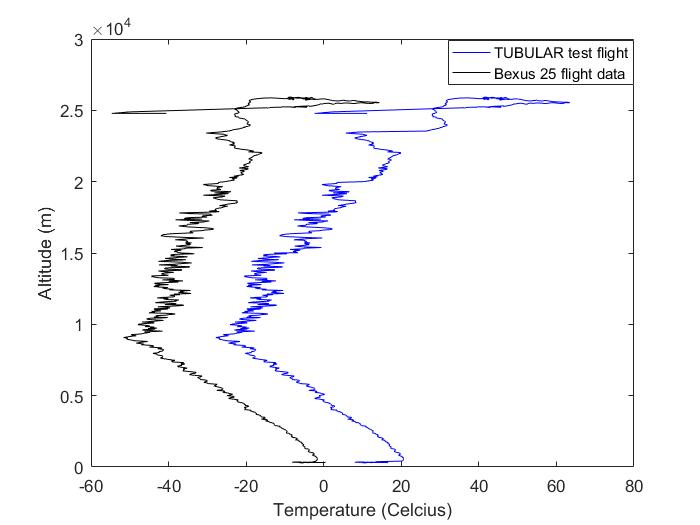
\includegraphics[width=1\linewidth]{appendix/img/Thermal/Real_test_flight_BEXUS_25.jpg}
    \end{align*}
    \caption{Simulated test flight of TUBULAR with data from BEXUS 25}
    \label{fig:thermal-testflight}
\end{figure}
When it have been found it were checked in ANSYS to determine and fix with heaters to control the most critical parts of the model thermal wise.

\subsubsection{Trial flight for the CAC}
\begin{figure}[H]
    \begin{align*}
        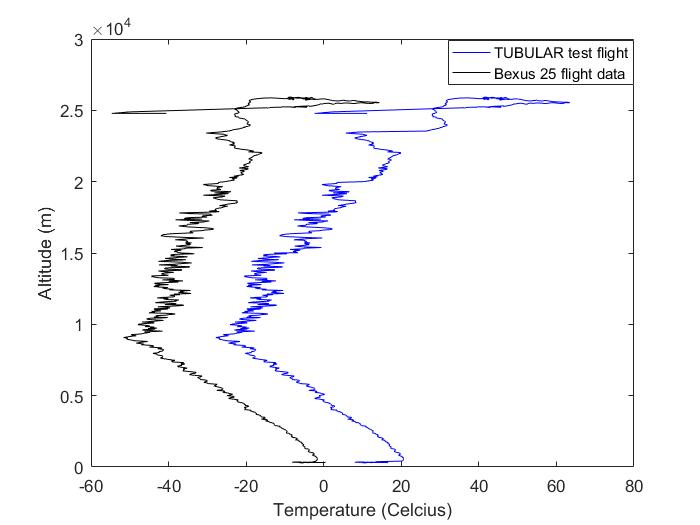
\includegraphics[width=1\linewidth]{appendix/img/Thermal/Real_test_flight_BEXUS_25.jpg}
    \end{align*}
    \caption{Simulated test flight of TUBULAR with data from BEXUS 25}
    \label{fig:thermal-testflight}
\end{figure}

\subsubsection{MATLAB conclusion}
By running the MATLAB script, the hotest and coldest case for $0.02m$ of styrofoam could be found for ascent and descent sampling. The thermal conductivity of styrofoam is $k=0.03$. In table \ref{tab:temperature-sampling-ascent-descent} it is shown the hottest and coldest case of temperature on the inside when samples should be taken. The hottest and coldest cases are taken from the figure \ref{fig:thermal-testflight}.


\begin{table}[H]
\centering
\label{tab:temperature-sampling-ascent-descent}
\begin{tabular}{|l|l|l|l|l|l|l|}
\hline
\multirow{2}{*}{Styrofoam thickness (m)} & \multirow{2}{*}{Inner area (m\textasciicircum{}2)} & \multirow{2}{*}{(L/kA)} & \multicolumn{2}{l|}{Coldest (C)} & \multicolumn{2}{l|}{Hottest (C)} \\ \cline{4-7} 
                                         &                                                    &                         & Ascent         & Descent         & Ascent         & Descent        \\ \hline
0.02                                     & 1.0692                                             & 0.6235                  & -7.592         & -20.47          & 19.91          & -0.5909        \\ \hline
\multicolumn{3}{|l|}{The outside air}                                                                                   & -38.22         & -44.41          & -15.9          & -31.18         \\ \hline
\end{tabular}
\caption{The temperature ranges for ascent and descent for $0.02m$ of styrofoam insulation}
\end{table}


\subsection{Thermal simulations ANSYS}
In ANSYS, FEA simulations were done by using both Steady-State Thermal and Transient Thermal.
Because of limitations of ANSYS student license a simplified model have been used, it can be seen in figure \ref{fig:Ansys-CAD-model}. It is in a lower corner with the components box and have three walls to the outside and the uniform air on the inside. The uniform inside air can be taken from the data from the test flight in figure (\ref{fig:thermal-testflight}). This simulations were done to see what temperature the pump and valves will be because they are the most critical components.

\begin{figure}[H]
    \begin{align*}
        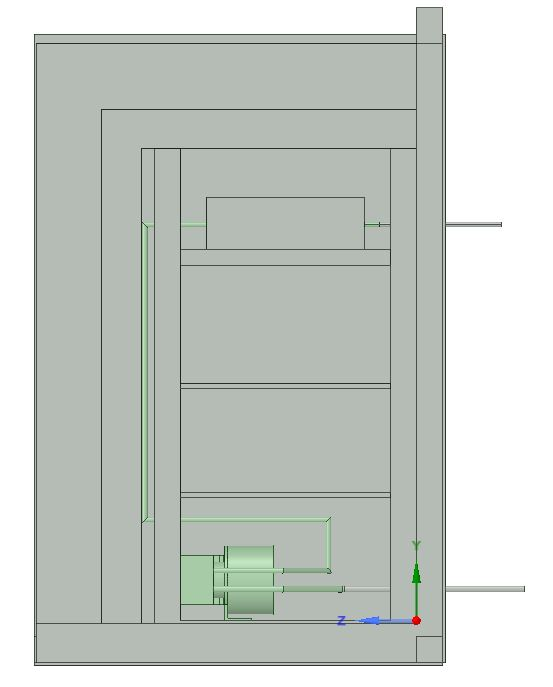
\includegraphics[width=0.5\linewidth]{appendix/img/Thermal/Thermal_CAD_model.JPG}
    \end{align*}
    \caption{The CAD model used for ANSYS simulations}
    \label{fig:Ansys-CAD-model}
\end{figure}

The CAD model is as seen in the figure \ref{fig:Ansys-CAD-model}. The side exterior walls are $0.02m$, the interior walls of the brain box to the bags are $0.03m$ and the top and bottom wall consist of $0.03m$ styrofoam as well. The outer parts of the pipes are set to stainless steel with a constant temperature (The same as the ambient outside). Tubes closest to the pump and the one going from pump to the manifold are set to air to simulate and be able to variate depending on the temperature outside and the pump heating up from the heater.

A transient thermal analyze were done simulating a test flight with data from BEXUS 25 using results from MATLAB. It were done so the thickness of the wall could be verified if it were good and to be able to add heaters. By being able to add heaters and move around, change strength and time on it is possible to fix so the pump and the valve manifold will be in their operating temperature ranges.

\begin{figure}[H]
    \begin{align*}
        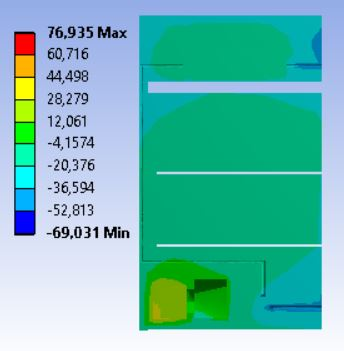
\includegraphics[width=0.5\linewidth]{appendix/img/Thermal/Ansys_simulation.JPG}
    \end{align*}
    \caption{Cross section of the air in the component box at the time to sample during ascent}
    \label{fig:Ansys-CAD-model}
\end{figure}

\begin{figure}[H]
    \centering
    \subfloat{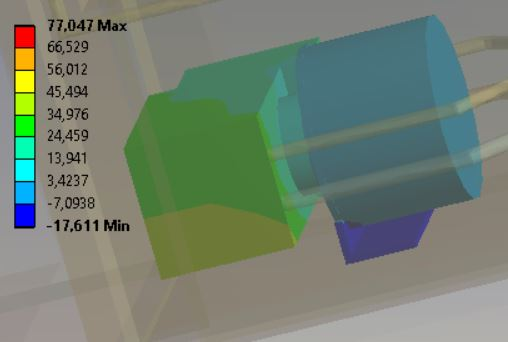
\includegraphics[width=0.4\linewidth]{appendix/img/Thermal/Pump_time_to_sample.JPG}}
    \hifll
    \subfloat{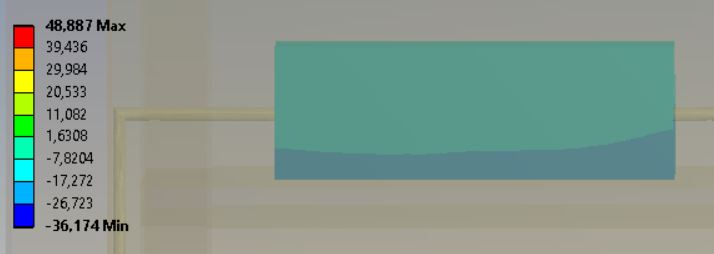
\includegraphics[height=0.21\linewidth]{appendix/img/Thermal/Valve_time_to_sample.JPG}}
    \caption{Pump and Valve at the time to sample during ascent}
    \label{fig:Pump-Valve-ascent-sample}
\end{figure}

\begin{figure}[H]
    \centering
    \subfloat{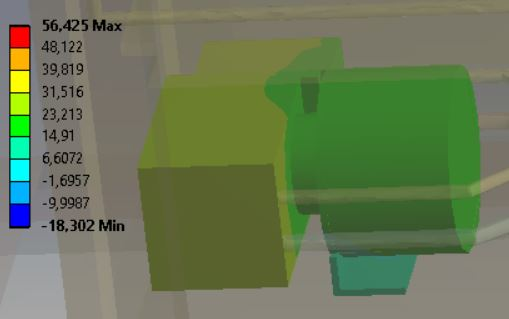
\includegraphics[width=0.4\linewidth]{appendix/img/Thermal/Pump_time_to_sample_descent.JPG}}
    \hifll
    \subfloat{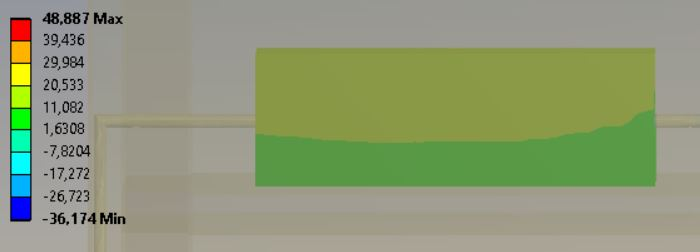
\includegraphics[height=0.21\linewidth]{appendix/img/Thermal/Valve_time_to_sample_descent.JPG}}
    \caption{Pump and Valve at the time to sample during descent}
    \label{fig:Pump-Valve-ascent-sample-descent}
\end{figure}

\subsection{Result}
The result from doing first MATLAB and then ANSYS have been to iterate to find the wall thickness of styrofoam between the brain box and the inside of the AAC box. Next step is to be able to determine what heaters and how many will be needed. By running a transient thermal analysis for the test flight there is the possible to simulate heaters that will be on and off to determine how strong they need to be.

The results from ANSYS simulations is assuming that it is the worst case. It gives that the results are not fully accurate but should be a bit warmer in reality. By looking at figure \ref{fig:Pump-Valve-ascent-sample} and \ref{fig:Pump-Valve-ascent-sample-descent}. The temperature can be seen and check for the pump to be above $5\degree C$ and the pump above $-10\degree C$. It is only during a little before ascent to the time for sample the heater should be on for the pump to get above $5\degree C$ and it is on during ascent. During descent it needs to be on a short period.

With an insulation of $0.02m$ styrofoam and $0.002m$ of aluminum sheets as outer wall. For the three inner walls between the brain box and the bags there will be a $0.03m$ wall of styrofoam. By using a 10W heater for the pump and one 10W heaters for the manifold. The critical components shall be working.

